\chapter{三角学回顾}
如图.\\
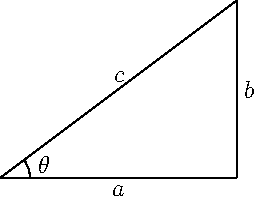
\includegraphics{triangel.pdf}

基本公式列表:
\begin{equation*}
\begin{array}{l l l}
    \displaystyle\sin(\theta)=\frac{b}{c} & \displaystyle\cos(\theta)=\frac{a}{c} & \displaystyle\tan(\theta)=\frac{b}{a}\\
    \displaystyle\csc(\theta)=\frac{1}{\sin(\theta)}=\frac{c}{b} & \displaystyle\sec(\theta)=\frac{1}{\cos(\theta)}=\frac{c}{a} & \displaystyle\cot(\theta)=\frac{1}{\tan(\theta)}=\frac{a}{b}
\end{array}
\end{equation*}
常见三角函数值:\\
\begin{equation*}
\begin{array}{>{\displaystyle}c|>{\displaystyle}c >{\displaystyle}c >{\displaystyle}c >{\displaystyle}c >{\displaystyle}c}
\hline
    & 0 & \frac{\pi}{6} & \frac{\pi}{4} & \frac{\pi}{3} & \frac{\pi}{2}\\[1ex]
\hline
    \sin & 0 & \frac{1}{2} & \frac{\sqrt{2}}{2} & \frac{\sqrt{3}}{2} & 1\\[1ex]
    \cos & 1 & \frac{\sqrt{3}}{2} & \frac{\sqrt{2}}{2} & \frac{1}{2} & 0\\[1ex]
    \tan & 0 & \frac{\sqrt{3}}{3} & 1 & \sqrt{3} & \star\\[1ex]
\hline
\end{array}
\end{equation*}\\

求三角函数值步骤:\\
1.找出角所在象限;\\
2.当角在x/y轴上, 参考三角函数图像;\\
3.如果角不在x/y轴上, 找出该角与x轴形成的最小角度, 即\textbf{参考角};\\
4.当参考角为特殊角时,参考常见三角函数值表;\\
5.利用ASTC(all/sin/tan/cos)决定是否需要添加负号.\\

例1.\\
\phantom{例1}$\displaystyle\sin(\frac{\pi}{4})$\\
1)$\frac{\pi}{4}$在第一象限, $\sin$值为正\\
2)与x轴形成的角为$\frac{\pi}{4}$\\
结果为:\\
$\displaystyle\sin\frac{\pi}{4}=\frac{\sqrt{2}}{2}$\\

例2.\\
\phantom{例2}$\displaystyle\cos(\frac{5\pi}{6})$\\
1)$\frac{5\pi}{6}$在第二象限, $\cos$值为负\\
2)与x轴形成的角为$\frac{\pi}{6}$\\
结果为:\\
$\displaystyle\cos\frac{5\pi}{6}=-\cos\frac{\pi}{6}=-\frac{\sqrt{3}}{2}$\\

例3.\\
\phantom{例3}$\displaystyle\tan(\frac{4\pi}{3})$\\
1)$\frac{4\pi}{3}$在第三象限, $\tan$值为正\\
2)与x轴形成的角为$\frac{\pi}{3}$\\
结果为:\\
$\displaystyle\tan\frac{4\pi}{3}=\tan\frac{\pi}{3}=\sqrt{3}$\\

例4.\\
\phantom{例4}$\displaystyle\cot(\frac{5\pi}{3})$\\
1)$\frac{5\pi}{3}$在第四象限, $\cot$值为负\\
2)与x轴形成的角为$\frac{\pi}{3}$\\
结果为:\\
$\displaystyle\cot\frac{5\pi}{3}=-\cot\frac{\pi}{3}=-\frac{\sqrt{3}}{3}$\\[2ex]

三角函数图像:\\
\begin{figure}[H]
\centering
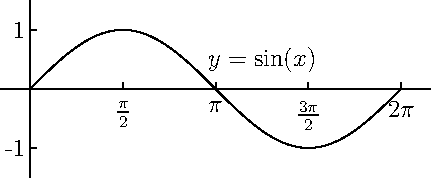
\includegraphics{sin.pdf}
\end{figure}
\begin{figure}[H]
\centering
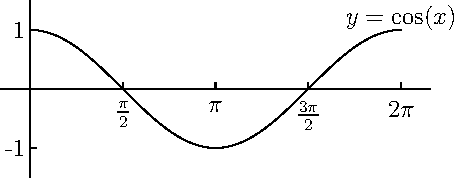
\includegraphics{cos.pdf}
\end{figure}
\begin{figure}[H]
\centering
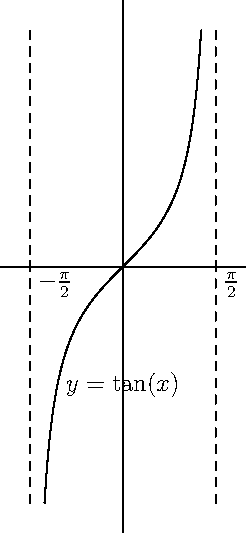
\includegraphics{tan.pdf}\qquad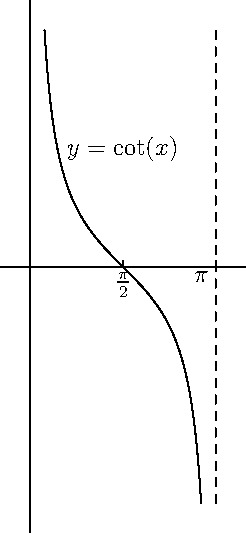
\includegraphics{cot.pdf}
\end{figure}
\begin{figure}[H]
\centering
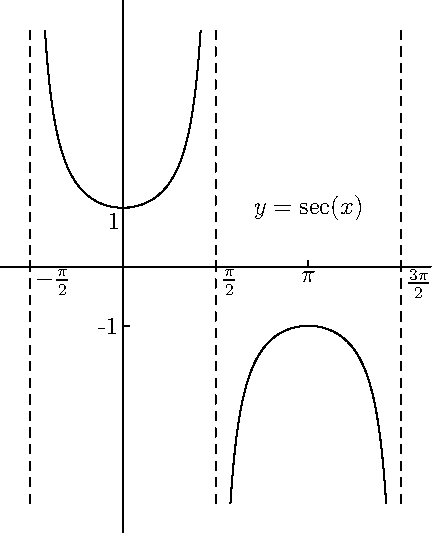
\includegraphics{sec.pdf}
\end{figure}
\begin{figure}[H]
\centering
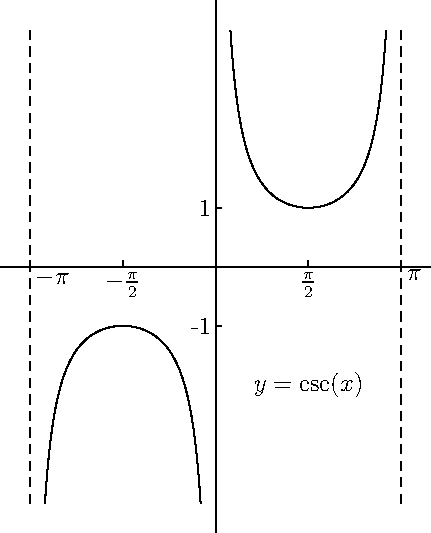
\includegraphics{csc.pdf}
\end{figure}

毕达哥拉斯定理:
{\par\centering
\framebox{$\cos^2(x)+\sin^2(x)=1$}
\par}

等式两边除以$\cos^2(x)$:
{\par\centering
\framebox{$1+\tan^2(x)=\sec^2(x)$}
\par}

等式两边除以$\sin^2(x)$:
{\par\centering
\framebox{$\cot^2(x)+1=\csc^2(x)$}
\par}

余角公式:
{\par\centering
    \framebox{$\cos(x)=\sin(\frac{\pi}{2}-x)$,$\cot(x)=\tan(\frac{\pi}{2}-x)$,$\csc(x)=\sec(\frac{\pi}{2}-x)$}\\[2ex]
    \framebox{$\sin(x)=\cos(\frac{\pi}{2}-x)$,$\tan(x)=\cot(\frac{\pi}{2}-x)$,$\sec(x)=\csc(\frac{\pi}{2}-x)$}
\par}

和/差角公式:
{\par\centering
    \framebox{$\sin(A+B)=\sin(A)\cos(B)+\cos(A)\sin(B)$}\\[2ex]
    \framebox{$\cos(A+B)=\cos(A)\cos(B)-\sin(A)\sin(B)$}\\[2ex]
    \framebox{$\sin(A-B)=\sin(A)\cos(B)-\cos(A)\sin(B)$}\\[2ex]
    \framebox{$\cos(A-B)=\cos(A)\cos(B)+\sin(A)\sin(B)$}
\par}

倍角公式:
{\par\centering
    \framebox{$\sin(2x)=2\sin(x)\cos(x)$}\\[2ex]
    \framebox{$\cos(2x)=\cos^2(x)-\sin^2(x)=2\cos^2(x)-1=1-2\sin^2(x)$}
\par}

%最后编辑于: 2021-12-30
